\documentclass[12pt]{article}

%% General
\usepackage{enumitem}
\usepackage{verbatim} 
\usepackage[utf8]{inputenc}

% URL
\usepackage{hyperref}

% Colour

\usepackage{xcolor}

\begin{comment}
%Header

\usepackage{fancyhdr}
\pagestyle{fancyplain}
\fancyhead{} % No page header - if you want one, create it in the same way as the footers below
\fancyfoot[L]{} % Empty left footer
\fancyfoot[C]{} % Empty center footer
\renewcommand{\headrulewidth}{0pt} % Remove header underlines
\renewcommand{\footrulewidth}{0pt} % Remove footer underlines
\setlength{\headheight}{0pt} % Customize the height of the header
\end{comment}


% Captions
\usepackage[margin=10pt,font=small,labelfont=bf, labelsep=endash]{caption}

%% Geometry

\usepackage[margin=1in]{geometry}


%% Maths

\usepackage[centertags]{amsmath}
\usepackage{amsfonts}
\usepackage{amssymb}
\usepackage{amsthm}
\usepackage{newlfont}

\theoremstyle{plain}
%\theoremstyle{margin}
{\swapnumbers
\newtheorem{thm}{Theorem}[section]
\newtheorem{cor}[thm]{Corollary}
\newtheorem{lem}[thm]{Lemma}
\newtheorem{prop}[thm]{Proposition}
}
%
\theoremstyle{definition}
%\newtheorem{defn}{Definition}[section]
%\newtheorem{nota}{Notation}[section]
%\theoremstyle{margin}
{\swapnumbers
\newtheorem{defn}[thm]{Definition}
\newtheorem{nota}[thm]{Notation}
\newtheorem{parag}[thm]{}
\newtheorem*{parstr}{\addtocounter{thm}{1}\thesection.\arabic{thm}*}
\newtheorem*{intropar}{\addtocounter{thm}{1}\arabic{thm}}
}
%
\theoremstyle{remark} {\swapnumbers
\newtheorem{rem}[thm]{Remark}
\newtheorem{exam}[thm]{Example}
\newtheorem{lemma}[thm]{Lemma}
\newtheorem{claim}[thm]{Claim}
}


%% Graphics
\usepackage{graphicx} 
\graphicspath{{Figures/}} 
\usepackage{subfig}

%% Tables
\usepackage{booktabs}
\usepackage{rotating}

% Allows shading of table cells
\usepackage{colortbl}

% Define a simple command to use at the start of a table row to make it have a shaded background
\newcommand{\gray}{\rowcolor[gray]{.9}}

%% Commands
\newcommand{\bd}{\textbf}
\newcommand{\itt}{\textit}
%
\newcommand{\al}{\alpha}
\newcommand{\be}{\beta}
\newcommand{\de}{\delta}
%
\newcommand{\To}{\longrightarrow}
\newcommand{\RE}{\operatorname{Re}}
\newcommand{\IM}{\operatorname{Im}}
%
\newcommand{\QQ}{\mathbb{Q}}     
\newcommand{\RR}{\mathbb{R}}      
\newcommand{\ZZ}{\mathbb{Z}}      
\newcommand{\CC}{\mathbb{C}}      

\numberwithin{equation}{section}

%% Title

\begin{comment}
\setlength{\droptitle}{-8em} 
\title{	
\normalfont \normalsize \bf
\vspace{-1 em}} 
\end{comment}

%% Referencing

\usepackage[style=nature]{biblatex}

\usepackage{float}
\graphicspath{ {images/} }
%
\addbibresource{bib.bib}
%
\begin{document}

\title{Classical Chaos and Quantum Chaology}
\author{Alexander Illarionov}
\date{June 20, 2015}
\maketitle
%
\section*{Introduction}
\par From shuttle buses and pedestrian flow\cite{shuttle} to the orbit of our Home\cite{nbody}, \itt{chaos} permeates human existence. Chaos is ubiquitous, and the \itt{sine qua non} elements of reality exhibit turbulent behaviour: quanta.\\\\
Chaos is a persisting instability which makes deterministic motion so sensitive to any perturbation that a prediction of its trajectory is limited.\cite{berry358} Although research on chaotic systems gave birth to theoretical and applied gems in mathematics and physics, quantum chaos remains a mystery rather than a well-established concept. There is no persistent exponential sensitivity of most\cite{berry230} quantum dynamical systems to initial conditions, but there are universal quantum phenomena which resonate chaos of homologous classical settings.\cite{berry191}\\\\
Correspondence of classical mechanics and quantum theory is not a novel idea. In the first quarter of the XX century grandfathers of modern physics, Max Planck and Albert Einstein, theoretically investigated quantum relatives of a simple pendulum: lasers.\cites{1900a}{1900b}{ein} In a laser the role of a flying bob is often played by a beam of protons or electrons, each rotating around an arbitrary axis in conformity with their spin. However, classical mechanics and quantum theory are fundamentally different despite the apparent relationship.\cite{qm1} First of all, the energy of a quantum harmonic oscillator is \itt{quantised}. Characteristic energy values, or \itt{eigenvalues}, of the wavefunction are discrete in a quantum system, but form a continuous spectrum in the classical setting. Secondly, the energy of a quantum system in its lowest stationary state, called the \itt{zero-point} energy, is greater than zero. The nonzero zero-point energy is a necessary condition for the oscillator to conform the Heisenberg uncertainty principle, since the null zero-point energy implies zero momentum and zero uncertainty in position.\cite{uni} The lowest energy of a classical harmonic oscillator, however, \itt{is} zero at rest in equilibrium.\\\\Discreteness of energy levels in quantum systems imposes a limit on their time development: only periodic motion with definite frequencies is allowed. Inconsistency of the limit with classical chaos evokes doubt about the validity of the \itt{correspondence principle} between classical mechanics and quantum theory.\cite{berry358} If quantum mechanics admits only regularity in motion, why do chaotic systems \itt{exist}? How is the chaotic behaviour of the classical system reflected in the quantum counterpart?
%
\section*{Classical Chaos}
\itt{Quantum chaology}  \cite{berry163} studies the relationship between chaotic and quantum systems. In order to understand what quantum chaos \itt{is}, it is necessary to learn how chaotic motion can be described. One of the tools of a quantum chaologist is a concept of \itt{phase space}, which dates back to Newton.\cites{gutz}{newt} In the second chapter of \itt{Principia Mathematica} Newton introduces axioms of motion; the second law establishes the direct proportionality of the force and change in momentum. The intuitive relationship given by Newton was later rigorously formalised by William Rowan Hamilton and Karl Gustav-Jacob Jacobi into the concept of phase space, which extends three dimensions of Euclidian space to six, three for momentum and three for position.\cite{meh, gutz}Momentum and position are \itt{complementary} quantities, which give the complete instantaneous information about a dynamical system.\cite{port} Visualisation of six dimensions is not easy, but in some cases, where symmetry or invariants are present, phase space can be reduced to manageable three or two dimensions. One of the systems in which the reduction is possible is that of a hydrogen atom, which consists of a lone electron around a lone proton.\cite{gutz}\\\\
The electron in a hydrogen atom is located in the 1s electron shell. For low principle quantum numbers, the difference between orbital energies is relatively high. For high enough principle quantum numbers, orbitals get closer together and the difference between their energies substantially decreases. Thus, if enough energy is supplied such that the electron in a hydrogen atom is excited to the higher energy level but not stripped from the proton, the energy levels in which the electron can be found form a continuum and the rules of classical mechanics apply.\cite{port}\\\\
Such an excited atom is called a \itt{Rydberg atom}. In a strong magnetic field a Rydberg atom exhibits chaotic character. The magnetic field introduces an axis of symmetry through the atomic nucleus, since almost all the motion of the electron occurs in a plane. The symmetry reduces the phase space to four dimensions. Moreover, the total energy of the isolated and closed system of a Rydberg atom does not change. By considering a particular energy value, the three-dimensional \itt{energy shell} of a phase space is obtained. The resultant space can then be projected on a fixed plane, called a \itt{Poincar\'e section}. A Poincar\'e section of the excited hydrogen atom is shown on page \pageref{fig:1}.\\\\
In classical dynamics, chaotic systems satisfy three conditions \cite{port}:
\begin{enumerate}
	\item Boundedness. There exists a ball of a sufficiently large finite radius which contains any chaotically moving element of the system.
	\item Infinite recurrence. For an element in a chaotic system an arbitrarily small neighbourhood around the initial point of its trajectory is visited infinitely many times.
	\item Exponential sensitivity. In a chaotic system for any elements emanating arbitrarily closely the trajectories diverge exponentially.  
\end{enumerate}
A dynamical system which satisfies the conditions 1 and 2 but not the condition 3 is called \itt{quasiperiodic}.\\\\
If atoms and molecules in the ground state are considered classically in the context of the \itt{n}-body problem, it can be shown that all of them except a hydrogen atom and other two-body atomic systems behave chaotically. \cite{atph} In the quantum dynamical setting, however, these systems do not exhibit classical chaos, yet the associated wavefunctions and eigenvalues are strongly influenced by the chaotic property of the classical counterpart.\\\\
A simple model of a classical dynamical system is that of a billiard point mass on a frictionless billiard table. \cite{zeev,sinai} A billiard table is a smooth bounded planar enclosure. A point mass reflects from its boundary with the angle of incidence equal to the angle of reflection. Depending on the angle of projection and the shape of the table boundary, the motion of a billiard is either periodic, quasiperiodic or chaotic.
\section*{Quantum Chaology in a Billiard Hall}
A classical billiard table can be \itt{quantised} to model a quantum system. The quantum mechanical description takes into account the wave-particle duality of a quantum dot replacing a point mass. To each energy level of a quantum system there corresponds a unique stationary state, called \itt{eigenstate}, which defines a time-invariant wavefunction of a particle. \cite{port} The eigenstate in a quantum system resembles a stationary wave pattern on a membrane of the drum. For some systems, which include an electron trapped inside a circular box, the spectrum of eigenvalues is readily determinable, which reflects regularity of the billiard table in the classical setting. However, when the corresponding classical system is chaotic, a different non-regular pattern of energy levels emerges(cf. Figure \ref{fig:2} on page \pageref{fig:2}).
\\\\Although patterns which arise in quantum billiards may look random, in the early 1980s Eric Heller found that the eigenstates tend to concentrate around narrow channels,called \itt{scars}, of enhanced eigenstate intensity. \cite{gutz, hellb} A series of eigenstates were calculated for a two-dimensional quantum billiard stadium with a chaotic classical counterpart. Surprisingly, similar patterns were discovered in the eigenstates of a Rydberg hydrogen atom, see Fig \ref{fig:3} on page \pageref{fig:3}.\\\\
The deep effect of classical dynamics seems to lie in the local statistics of the energy spectrum, such as the \itt{level spacing distribution}.\cite{zeev}The level spacing distribution is the distribution of all distances between successive energy levels. In the study of quantum chaology the following open \itt{universality conjectures} were proposed, which seem to hold for most systems of the \itt{generic case}\cite{pr}:
\begin{enumerate}
\item If the classical system is not chaotic, then the level spacing distribution coincides with the corresponding distribution of \itt{uncorrelated}, or random, energy levels with the same mean spacing.\cite{tabor}
\item If the classical system is chaotic, then the level spacing distribution coincides with the corresponding distribution of a suitable \itt{ensemble} of random matrices, which define completely the properties of the physical system. \cite{BGS}
\end{enumerate}
In the 1960s Martin Gutzwiller introduced another tool of quantum chaology: the formalism of quantisation by periodic orbits.\cite{port, gut}  The kernel of the method is \itt{Gutzwiller's trace formula} which directly relates classical chaos and quantum mechanics.\cite{pr} One side of the trace formula combines lengths of closed chaotic orbits in the classical dynamical system, while the other involves a combination of the eigenvalues in the quantum system. Thus, by considering characteristics of chaos in the classical setting, properties of the corresponding quantum system can be deduced without solving the Schr\"{o}dinger equation. Asymptotic approximation of the solution to the Schr\"{o}dinger equation by the trace formula, however, is not random. Gutzwiller's approach matches another method of solving the same problem: Feynman's path approach.\cite{pr}
\section*{Conclusion}
Classical chaos and quantum theory are closely related, but the relationship is not yet well-defined. One can be studied with the help of the other in the field of \itt{semiclassical} physics. The semiclassical limit, in which the connection is the most apparent, is subtle, and more conundrums remain unsolved than concepts established to the present day. Although significant progress have been made in the last decades, fundamental questions of quantum chaology stand unanswered:
\begin{itemize}
\item How does order of the classical system affect the intrinsic properties of the quantum analogue?
\item Does the present definition of chaos contain all the necessary and sufficient conditions accounting for its connection with quantum mechanics?
\item Why do the statistics of the random matrix ensembles describe accurately the experimental fluctuations of energy levels?
\end{itemize}
The field of quantum chaology is still in its infancy. Research in chaos has become more active in the past 20 years due to the unexpected connection between distribution of energy levels in the quantum systems with classically chaotic analogues and one of the most important functions in mathematics, Riemann zeta function. Insights are yet to come. Stay tuned. 
\newpage
\section*{Appendix I}
\begin{figure}[H]
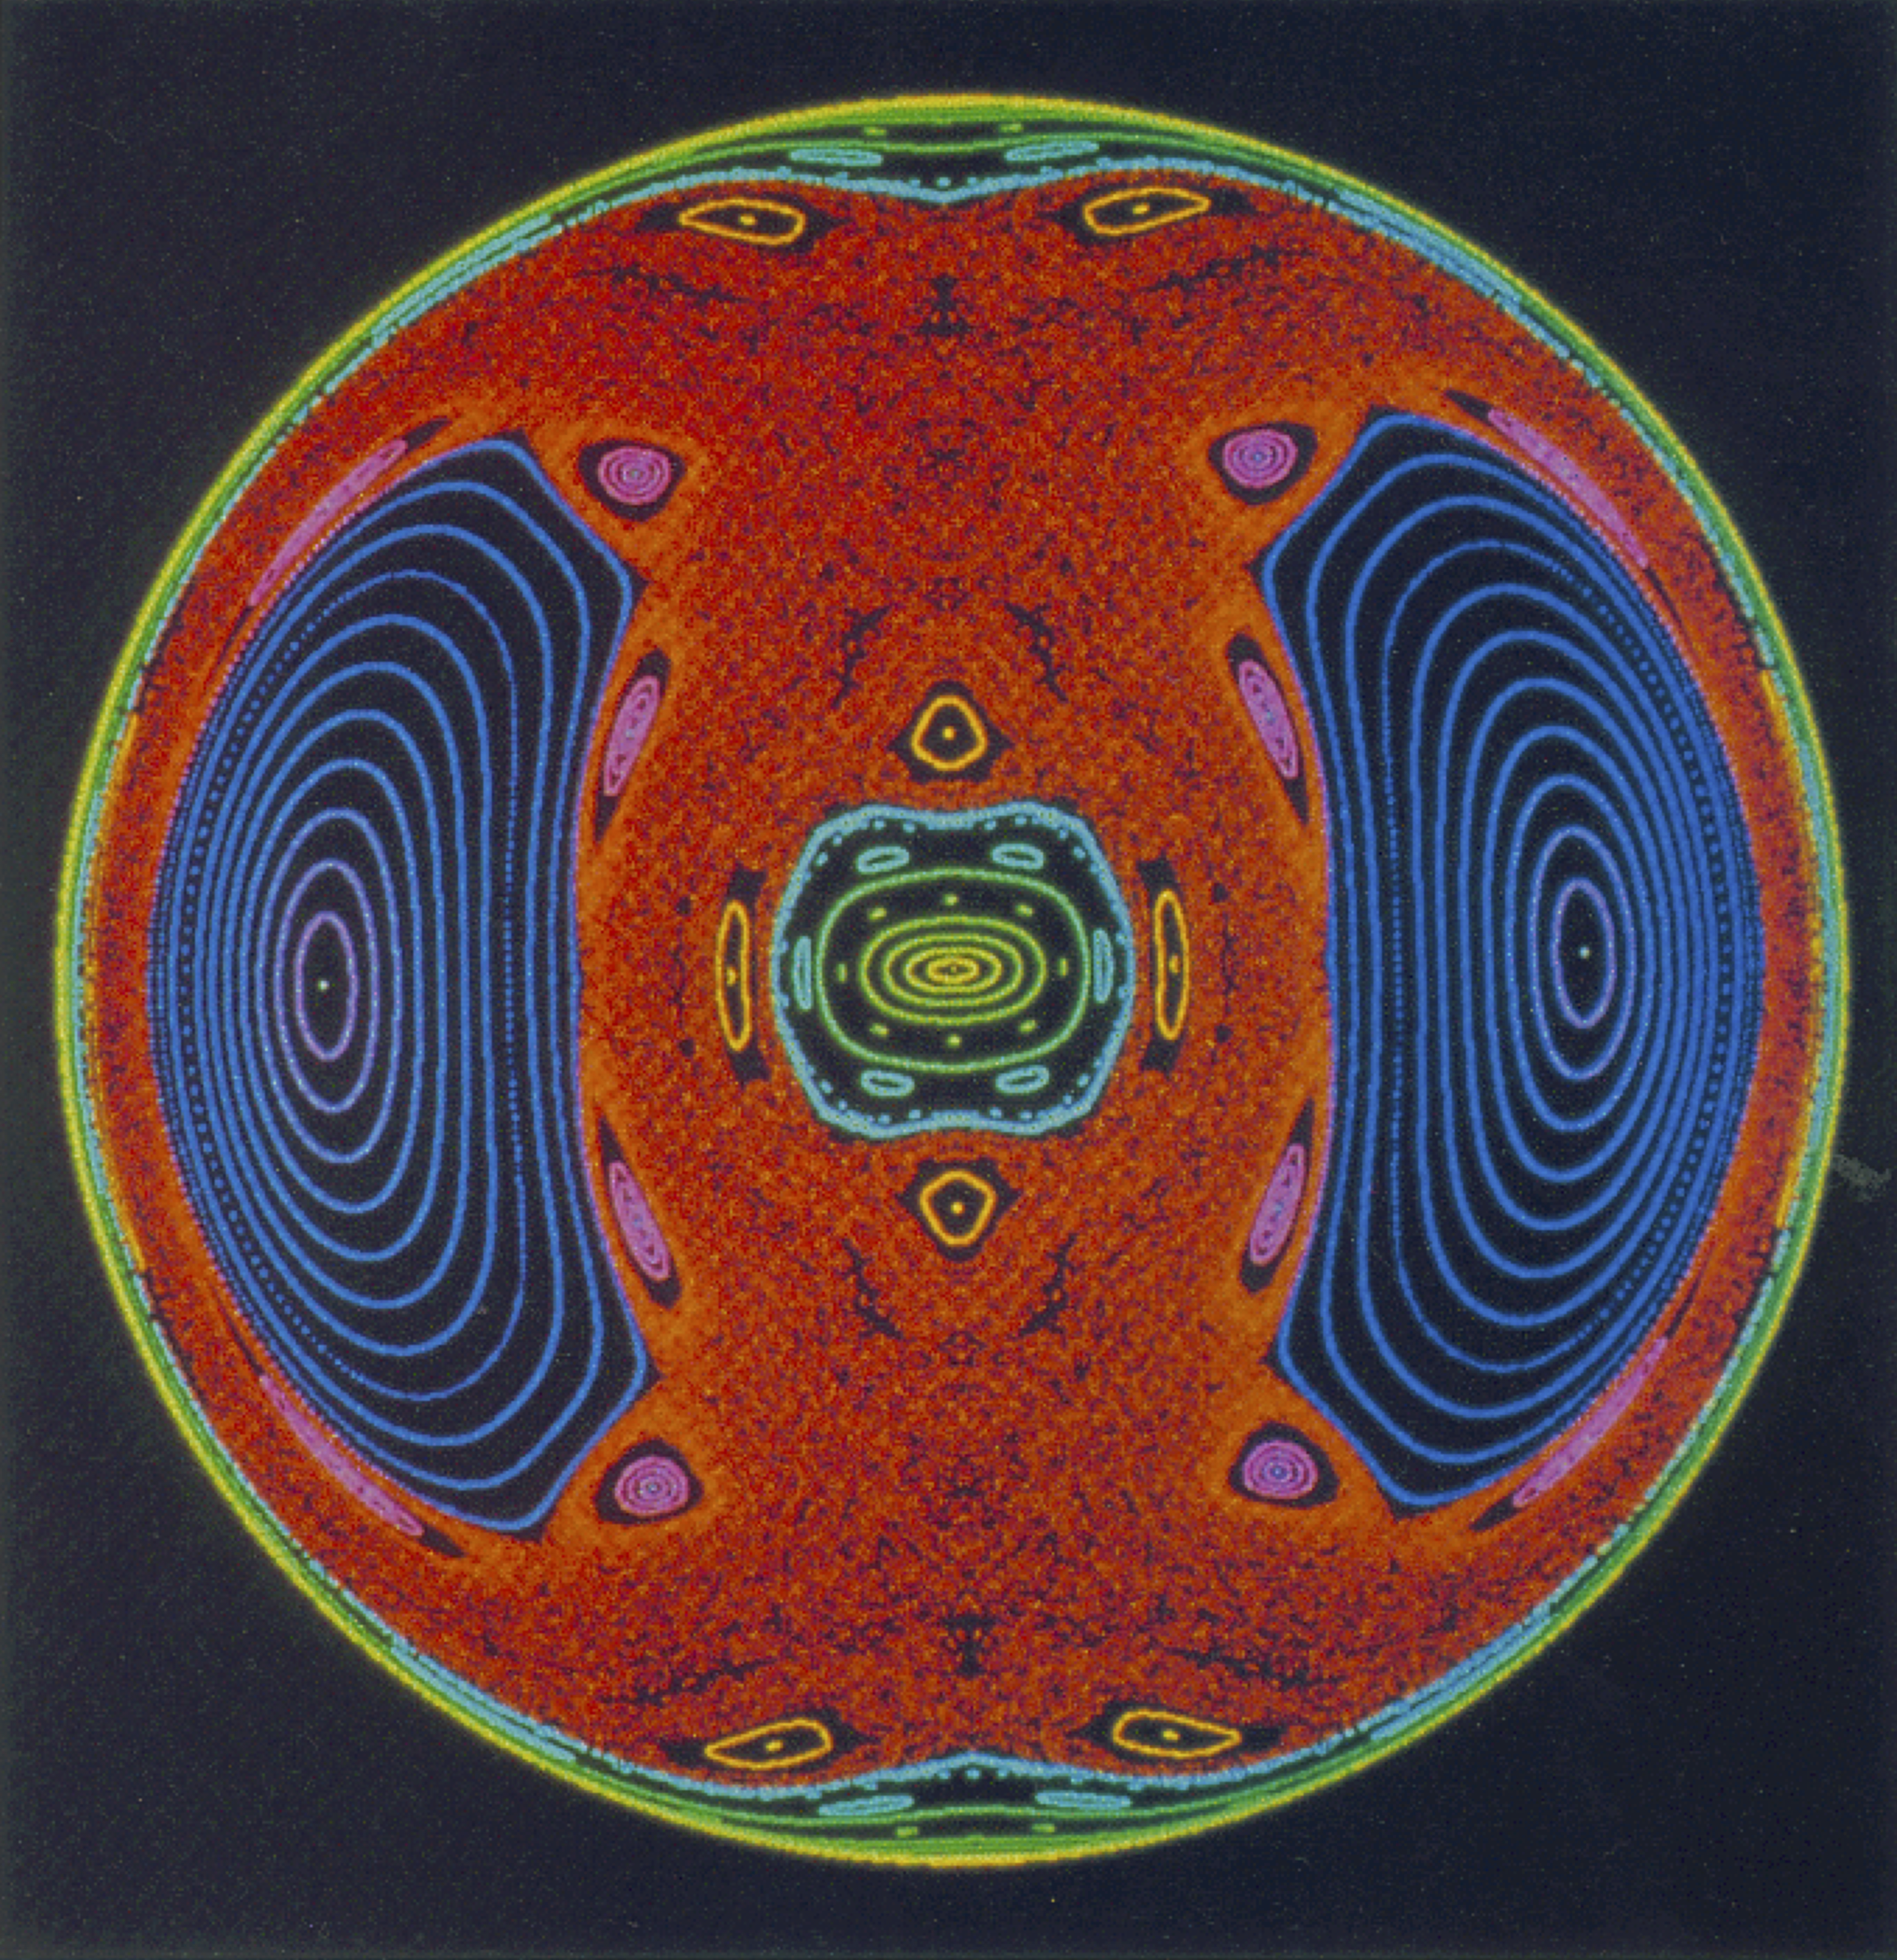
\includegraphics[width=\textwidth]{1}
\caption{The Poincar\'e section of the excited hydrogen atom indicates chaotic behaviour of the electron in the regions where the points of its trajectory scatter chaotically, shown in orange. Credit:\cite{gutz}}
\label{fig:1}
\end{figure}
\section*{Appendix II}
\begin{figure}[H]
\includegraphics[width=\textwidth]{2}
\caption{Left: classical orbits of a point mass in classical billiards.Right: corresponding waves of quantum billiards. Credit:\cite{berry358}}
\label{fig:2}
\end{figure}
\section*{Appendix III}
\begin{figure}[H]
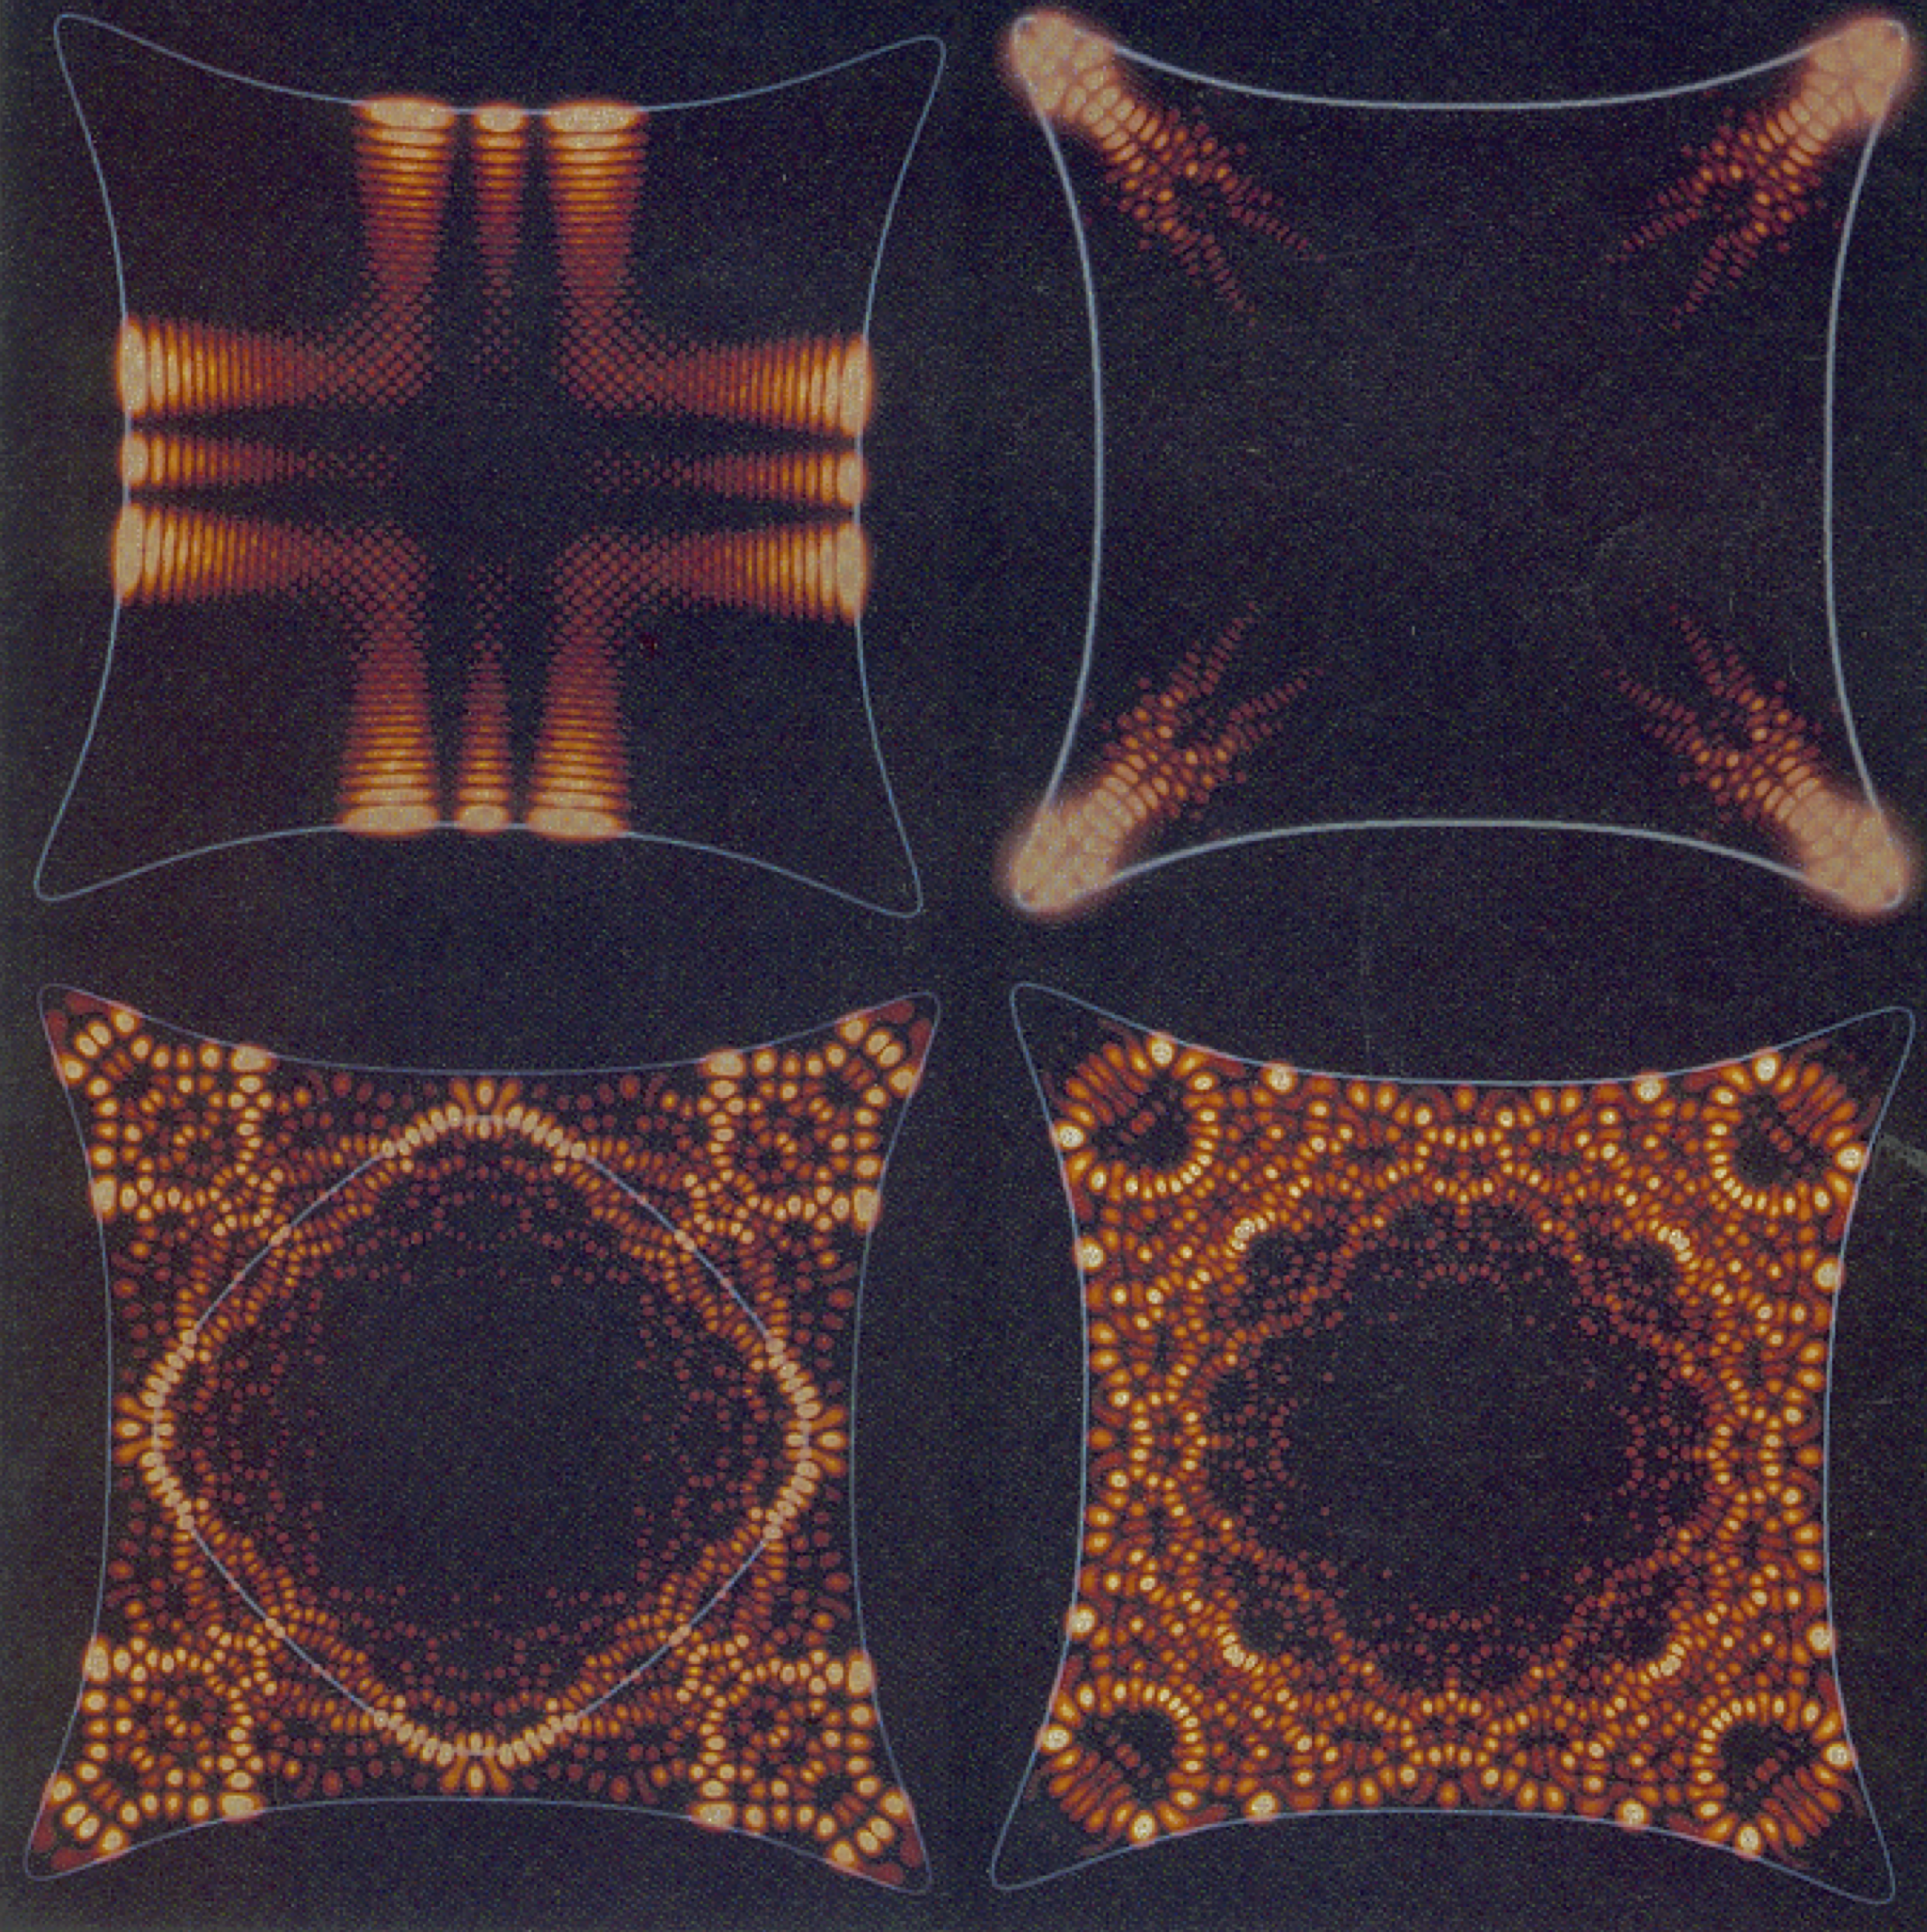
\includegraphics[width=\textwidth]{3}
\caption{Top: seemingly regular eigenstates of a Rydberg hydrogen atom. Bottom: \itt{scarring} characteristic for classically chaotic billiards. Credit:\cite{gutz}}
\label{fig:3}
\end{figure}
\newpage
%
\printbibliography
%
\end{document}